% !TeX document-id = {85e2339c-8979-4e3c-b8f8-e83964bef4d8}
% !TeX TXS-program:compile = txs:///pdflatex/[--shell-escape]
% ----------------------- TODO ---------------------------
% Diese Daten müssen pro Blatt angepasst werden:
%\newcommand{\NUMBER}{1}
\newcommand{\EXERCISES}{5}
% Diese Daten müssen einmalig pro Vorlesung angepasst werden:
%\newcommand{\COURSE}{Theoretische Informatik}
%\newcommand{\TUTOR}{Vorname Nachname}
%\newcommand{\STUDENTA}{John Doe}
%\newcommand{\STUDENTB}{Jane Doe}
%\newcommand{\STUDENTC}{Max Mustermann}
%\newcommand{\DEADLINE}{XX.0X.2019}
% ----------------------- TODO ---------------------------

\documentclass{uebungsblatt}

%\usepackage{uebungsblatt}

\begin{document}

% Hier nichts ändern
\maketitle


%------------------------------------------------------------------------------
%     START: Our Command & Environment Usage
%------------------------------------------------------------------------------

\section*{Unsere Spielereien}

\subsection*{Commands}
\subsubsection*{newcommand}
\hello \\
\hello[Jules]

\subsubsection*{renewcommand}
\noindent
$\Box\square$


\subsection*{Environments}

\begin{para}{Lorem Ipsum Text}
    \lipsum[2-3]
\end{para}


\begin{joke}
    Wie heißt ein weißes Mammut?\\
    \textbf{Helmut!}
\end{joke}

\begin{joke}
    Was macht ein Mathematiker beim Skifahren?\\
    \textbf{Er rechnet mit Brüchen!}
\end{joke}

\noindent
Es wurden \thejoke~ Witze gemacht!


\subsection*{Aufgaben:\quad Commands und Environments}
\begin{itemize}
    \item Natürliche Zahlen: $\bbN$
    \item Ganze Zahlen: $\bbZ$
    \item Rationale Zahlen: $\bbQ$
    \item Reelle Zahlen: $\bbR$
    \item Komplexe Zahlen: $\bbC$
\end{itemize}

\[\bbN \subset \bbZ \subset \bbQ \subset \bbR \subset \bbC\]

\aufgabe{42}{5}
Hier steht eine Aufgabenstellung Bliblablub.

\begin{loesung}
    \lipsum[5]
\end{loesung}

\noindent
Hier steht anderer Text. \lipsum[2]


\subsection*{Fonts}

%\familydefault     % Herausfinden welche FontFamily benutzt wird

% Slide 27
Hier steht was.
{\fontfamily{ComicNeue-TLF}\selectfont Hier Comic Neue.}
Hier wieder nicht.

% Slide 28
{\noindent\comicneue Hier steht etwas auf diese Weise} \\
\textcn{Hier steht etwas auf die andere Weise}


\subsection*{Aufgaben:\quad Fonts}

% Aufgabe 4: Monospace
\texttt{Hier steht was in Fira Mono!}

% Aufgabe 5: Awesome Fonts
\begin{figure}[h!]
    \centering
    {\Huge \faAd\ \faWikipediaW\ \faEnvelopeOpen[regular]\ \faSleigh\ \faOtter\ \faMicroscope\ \faEyeDropper}
    \caption{A.W.E.S.O.M.E.}
\end{figure}





\newpage
%------------------------------------------------------------------------------
%     END: Our Command & Environment Usage
%------------------------------------------------------------------------------


% ----------------------- TODO ---------------------------
% Hier werden die Aufgaben/Lösungen eingetragen:


\section*{Aufgabe 1}
\subsection*{a) Erstellung von Dokumenten mit LaTeX}

Dies ist eine Aufgabe. Text könnt ihr hier einfach ganz normal schreiben, jedoch bricht
Latex
nicht
die
Zeilen
um, wenn ihr im Editor eine neue Zeile anfangt.
Um einen Zeilenumbruch \\
zu erhalten \\
verwendet zwei Backslash.\\
Einen neuen Absatz erhaltet ihr, wenn ihr zwei Zeilenumbrüche einfügt.

Es gibt zwei Arten des Mathemodus, einen im Text $x_1 = 5 \cdot 10^{42}$ und einen 
freistehenden.

\[x_2 = \sqrt{ \sin{ \alpha \times \beta} \cdot \frac{a}{b}} + \log_2{64}\]

Wenn der Mathemodus sich über mehrere Zeilen erstrecken soll, so könnt ihr die 
Umgebung align benutzen. Der Stern sagt hierbei, dass die Zeilen nicht nummeriert 
werden sollen. Das \& ist ein align-parameter, die Zeilen werden hierbei so ausgerichtet, 
dass die \& immer über einander stehen.

\begin{align*}
\text{Text im Mathemodus} & = 5\\
x_2 &= 7\\
\Sigma + \phi + \epsilon + w &= \text{sinnlose Zeichen}
\end{align*}

Mengenklammern, die sich an der Größe des inneren orientieren, kann man so erzeugen
\[\left\{ \frac{2}{3} \cdot x \ \middle| \ x \in \mathbb{R} \right\} .\]


Ein Bild kann man folgendermaßen einbinden: \\
Entfernt dabei das \% und ersetzt Bild.jpg mit dem Dateinamen. \% kommentiert 
eine Zeile aus.

\begin{figure}[H]
\centering
%\includegraphics[width=11cm]{Bild.jpg}
\caption{Dies ist die Bildunterschrift}
\end{figure}

Eine Tabelle könnt ihr so anlegen:\\
In der zweiten geschweiften Klammer wird das Layout der Tabelle definiert. 
Das \& trennt hierbei die Spalten.\\
\ \\ %Trick um eine leere Zeile zu erhalten, 
     %gleichzeitig wird in der nächsten Zeile kein neuer Absatz begonnen
\begin{tabular}{c|lr}
  zentrierte Spalte & linksbündig & rechtsbündig\\
  \hline
  zweite Zeile & \\
\end{tabular}\\
\ \\
Eine neue Seite wird durch $\backslash$newpage erzwungen.
\newpage

Das hier ist eine nummerierte Aufzählung
\begin{enumerate}
\item Erster Punkt
\item Zweiter Punkt
\end{enumerate}

und das hier ist eine Aufzählung ohne Nummerierung
\begin{itemize}
\item Erster Punkt
\item Zweiter Punkt
\end{itemize}

\subsection*{b) Zeichnen von Automaten}

Übergangsrelationen von Automaten können ihr mit dem Tool auf
\url{http://madebyevan.com/fsm/} zeichnen. 

Alternativ, wenn ihr mehr Kontrolle über die Platzierung der Nodes haben wollt, 
könnt ihr die Übergangsrelationen auch ohne das Tool direkt in TikZ definieren,
siehe das Beispiel: \url{http://texample.net/tikz/examples/state-machine/}
\begin{center}
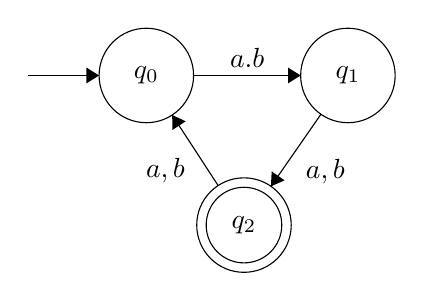
\begin{tikzpicture}[scale=0.2]
\tikzstyle{every node}+=[inner sep=0pt]
\draw [black] (18.5,-19.9) circle (3);
\draw (18.5,-19.9) node {$q_0$};
\draw [black] (31.3,-19.9) circle (3);
\draw (31.3,-19.9) node {$q_1$};
\draw [black] (24.7,-29.4) circle (3);
\draw (24.7,-29.4) node {$q_2$};
\draw [black] (24.7,-29.4) circle (2.4);
\draw [black] (11,-19.9) -- (15.5,-19.9);
\fill [black] (15.5,-19.9) -- (14.7,-19.4) -- (14.7,-20.4);
\draw [black] (21.5,-19.9) -- (28.3,-19.9);
\fill [black] (28.3,-19.9) -- (27.5,-19.4) -- (27.5,-20.4);
\draw (24.9,-19.4) node [above] {$a.b$};
\draw [black] (29.59,-22.36) -- (26.41,-26.94);
\fill [black] (26.41,-26.94) -- (27.28,-26.56) -- (26.46,-25.99);
\draw (28.6,-26.01) node [right] {$a,b$};
\draw [black] (23.06,-26.89) -- (20.14,-22.41);
\fill [black] (20.14,-22.41) -- (20.16,-23.36) -- (21,-22.81);
\draw (20.98,-25.97) node [left] {$a,b$};
\end{tikzpicture}
\end{center}

\subsection*{c) Pseudocode}

\begin{algorithm}
  \caption{Zähle die Anzahl der Stellen, an der zwei Binärzahlen sich unterscheiden}
  \begin{algorithmic}[1]
    \Require{$x$ und $y$ sind Binärzahlen der gleichen Länge}
    \Statex
    \Function{Distance}{$x, y$}
      \Let{$z$}{$x \oplus y$} \Comment{$\oplus$: bitweise exkulsives oder}
      \Let{$\delta$}{$0$}
      \For{$i \gets 1 \textrm{ to } n$} \Comment{$n$: Länge von $z$}
        \If{$z_i \neq 0$} \Comment{$z_i$: $i$tes Bit von $z$}
          \Let{$\delta$}{$\delta + 1$}
        \EndIf
      \EndFor
      \State \Return{$\delta$}
    \EndFunction
  \end{algorithmic}
\end{algorithm}
\end{document}
%%% Local Variables:
%%% mode: latex
%%% TeX-master: t
%%% End:
